\documentclass{article}
\usepackage[margin=1in]{geometry}
\usepackage{amsmath}
\usepackage{listings}
\usepackage{color}
\usepackage{graphicx}
\usepackage{blkarray}
\usepackage{multirow}

\definecolor{dkgreen}{rgb}{0,0.6,0}
\definecolor{gray}{rgb}{0.5,0.5,0.5}
\definecolor{mauve}{rgb}{0.58,0,0.82}

\lstset{frame=tb,
  language=Python,
  aboveskip=3mm,
  belowskip=3mm,
  showstringspaces=false,
  columns=flexible,
  basicstyle={\small\ttfamily},
  numbers=none,
  numberstyle=\tiny\color{gray},
  keywordstyle=\color{blue},
  commentstyle=\color{dkgreen},
  stringstyle=\color{mauve},
  breaklines=true,
  breakatwhitespace=true,
  tabsize=3
}

\begin{document}
\begin{titlepage}
	\setlength{\parindent}{0pt}
	\large

\vspace*{-2cm}

University of Waterloo \par
Econ 424 \par
2023-11-20 \par
\vspace{0.05cm}
Anonymized Usernmae: IJustWannaPass
\vspace{0.2cm}

{\huge Prediction Competition \# 6 \par}
\hrule

\vspace{1cm}
\textbf{Q1)} To solve this problem I did two things. The first was I encoded each word into a 300 length vector, I then made sentences by summing each element in the vector with each other. I did this for the pros, cons and headline. For the job title, and company I just encoded them using an integer. \\\\

Once I was done with preprocessing, I used a CNN comprised of 4 fully connected layers (dense) and one drop out layer to avoid over fitting. The $MSE$ and $R^2$ of the model is provided below:

\[ MSE = 1.1986 \]
\[ R^2 = 0.0018 \]

However the test accuracy was:

\[ Accuracy = 0.4262 \]

The layout of the model is provided below: \\
\begin{lstlisting}
_________________________________________________________________
 Layer (type)                Output Shape              Param #   
=================================================================
 dense (Dense)               (None, 1024)              927744    
                                                                 
 dense_1 (Dense)             (None, 512)               524800    
                                                                 
 dense_2 (Dense)             (None, 64)                32832     
                                                                 
 dropout (Dropout)           (None, 64)                0         
                                                                 
 dense_3 (Dense)             (None, 5)                 325       
                                                                 
=================================================================
\end{lstlisting}

\newpage

\textbf{Q2)} For the first figure, I have graphed the average feature value for the test and training set. Note that this only includes certain features, as the word2vec representation would be too big to reproduce on one graph:

\begin{tabular}{ll}

 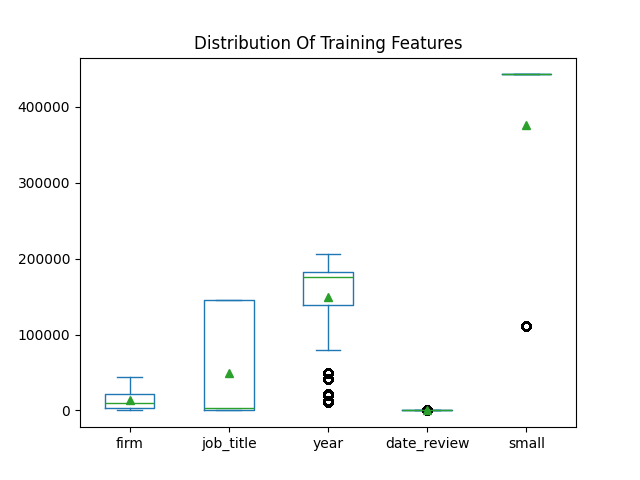
\includegraphics[width=.5\linewidth]{q1train.png} &  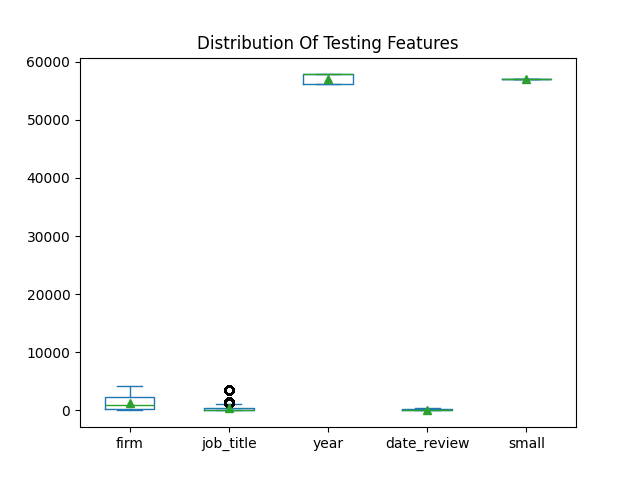
\includegraphics[width=.5\linewidth]{q1test.png}\\
 \hfil (i) Distribution of unique training observations  \hfil & \hfil (ii) Distribution of unique testing observations \hfil \\\\
 
\end{tabular}

We can see that in the testing set we are only dealing with a single type of year, and that the job titles are alot more spread out. In the next graph we can see the difference in distributions between the training data, predicted on the entire training data and predicted on the test data:
\begin{center}
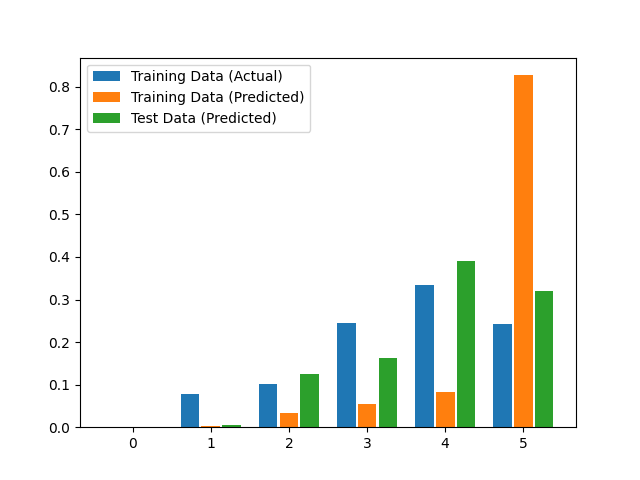
\includegraphics[width=.7\linewidth]{graph.png}
\end{center}
Finally we have a graph to demonstrate the covariance between the features which is displayed below:
\begin{center}
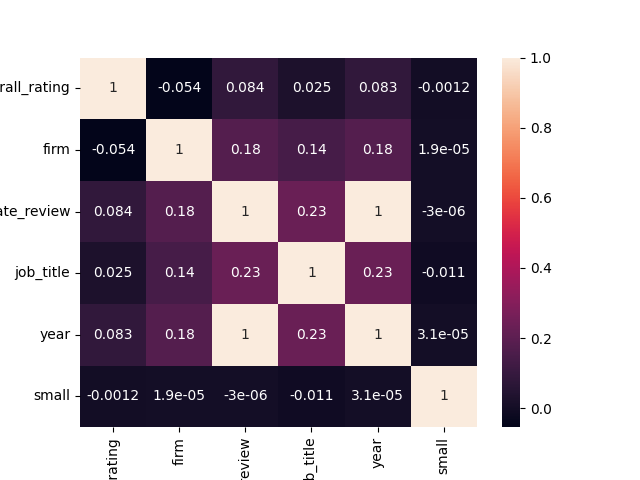
\includegraphics[width=.7\linewidth]{corr.png}
\end{center}
\newpage
\textbf{Q3)} To solve Q1 chatGPT was given the prompt: 
\begin{verbatim}
  Given a csv of Glassdoor reviews, create a CNN which can predict review ratings based on the 
  feature data
\end{verbatim}
chatGPT provided the following response:
\begin{verbatim}
Creating a Convolutional Neural Network (CNN) for predicting review ratings from a CSV file involves several steps. Here's a high-level outline of the process using Python and popular libraries like TensorFlow and Keras:

Import Libraries:

import pandas as pd
import numpy as np
from sklearn.model_selection import train_test_split
from sklearn.preprocessing import StandardScaler
from sklearn.preprocessing import LabelEncoder
from tensorflow.keras.models import Sequential
from tensorflow.keras.layers import Embedding, Conv1D, GlobalMaxPooling1D, Dense, Flatten
Load and Preprocess Data:


# Load CSV data
df = pd.read_csv('glassdoor_reviews.csv')

# Preprocess the data (you may need to adjust this based on your specific data)
X = df['feature_data_column'].values
y = df['rating_column'].values

# Use LabelEncoder to convert categorical labels to numerical
label_encoder = LabelEncoder()
y = label_encoder.fit_transform(y)

# Split the data into training and testing sets
X_train, X_test, y_train, y_test = train_test_split(X, y, test_size=0.2, random_state=42)

# Standardize the data (optional but often recommended)
scaler = StandardScaler()
X_train = scaler.fit_transform(X_train)
X_test = scaler.transform(X_test)
Tokenize Text Data:
In the case of textual features, you may need to tokenize and pad sequences. This step is specific to NLP tasks.


from tensorflow.keras.preprocessing.text import Tokenizer
from tensorflow.keras.preprocessing.sequence import pad_sequences

tokenizer = Tokenizer(num_words=vocab_size, oov_token="<OOV>")
tokenizer.fit_on_texts(X_train)
X_train = tokenizer.texts_to_sequences(X_train)
X_test = tokenizer.texts_to_sequences(X_test)

X_train = pad_sequences(X_train, maxlen=max_length, padding='post', truncating='post')
X_test = pad_sequences(X_test, maxlen=max_length, padding='post', truncating='post')
Build CNN Model:
model = Sequential()
model.add(Embedding(input_dim=vocab_size, output_dim=embedding_dim, input_length=max_length))
model.add(Conv1D(filters=128, kernel_size=5, activation='relu'))
model.add(GlobalMaxPooling1D())
model.add(Dense(128, activation='relu'))
model.add(Dense(num_classes, activation='softmax'))

model.compile(optimizer='adam', loss='sparse_categorical_crossentropy', metrics=['accuracy'])
Train the Model:
model.fit(X_train, y_train, epochs=num_epochs, validation_data=(X_test, y_test))
Evaluate the Model:

loss, accuracy = model.evaluate(X_test, y_test)
print(f'Test Loss: {loss:.4f}, Test Accuracy: {accuracy:.4f}')
Make Predictions:

predictions = model.predict(X_test)
Make sure to adjust hyperparameters, architecture, and other details based on your specific dataset and requirements. This is a basic outline to get you started, and you might need to tailor it further to fit your specific use case.







\end{verbatim}
\newpage
To solve Q2 chatGPT was given the prompt:
\begin{verbatim}
Produce a graph that shows the distribution of each feature in 
the training set and in the test
set.

Produce a second graph that shows 1) the distribution of predictions in the training set, (2) distribution of
actual values in training set and (3) distribution of predictions in the test set.

Produce a third graph that shows the correlation between each feature and between each feature and the
response variable in the training set. This can be a correlation heat-map or a more detailed visual presen-
tation
\end{verbatim}
chatGPT provided the following response: 
\begin{verbatim}
To create the requested graphs, you can use libraries such as matplotlib and seaborn for visualization and pandas for data manipulation. Below, I'll provide you with some example code snippets for each of the three graphs:

Graph 1: Distribution of Features in Training and Test Sets
python
Copy code
import matplotlib.pyplot as plt
import seaborn as sns

# Assuming X_train and X_test are your feature matrices
train_df = pd.DataFrame(X_train, columns=df.columns)  # Use your actual column names
test_df = pd.DataFrame(X_test, columns=df.columns)  # Use your actual column names

# Plot distribution of each feature in the training set
plt.figure(figsize=(15, 8))
plt.title('Distribution of Features in Training Set')
sns.boxplot(data=train_df)
plt.xticks(rotation=45, ha='right')
plt.show()

# Plot distribution of each feature in the test set
plt.figure(figsize=(15, 8))
plt.title('Distribution of Features in Test Set')
sns.boxplot(data=test_df)
plt.xticks(rotation=45, ha='right')
plt.show()
Graph 2: Distribution of Predictions and Actual Values in Training and Test Sets
python
Copy code
# Assuming 'predictions' is the output of model.predict on your test set

# Plot distribution of predictions and actual values in the training set
plt.figure(figsize=(12, 6))
sns.kdeplot(predictions, label='Predictions (Test Set)')
sns.kdeplot(y_test, label='Actual Values (Test Set)')
plt.title('Distribution of Predictions and Actual Values in Test Set')
plt.xlabel('Rating')
plt.ylabel('Density')
plt.legend()
plt.show()
Graph 3: Correlation Heatmap
python
Copy code
# Assuming 'df' is your training dataset with both features and response variable
correlation_matrix = df.corr()

# Plot correlation heatmap
plt.figure(figsize=(12, 10))
sns.heatmap(correlation_matrix, annot=True, cmap='coolwarm', fmt=".2f")
plt.title('Correlation Heatmap')
plt.show()
Make sure to replace 'feature_data_column', 'rating_column', and other placeholder names with your actual column names. Additionally, adjust the figure sizes, titles, and other parameters based on your preferences and the characteristics of your data.
\end{verbatim}
\end{titlepage}
\textbf{Code for Q1:}
\begin{lstlisting}
import tensorflow as tf
import numpy as np
import sklearn
import pandas as pd
import re
import gensim


from tensorflow.keras import layers, models
from gensim.models import KeyedVectors
from sklearn import metrics

dataset = pd.read_csv("Econ424_F2023_PC6_glassdoor_training_large_v1.csv")

firmDict = {}
jobTitleDict = {}
sentences = []


def convertString(string):
    return (''.join(ch for ch in string if ch.isalnum())).lower()


def updateDicts(row):
    firm = row["firm"]
    job = row["job_title"]

    firm = convertString(firm)
    job = convertString(job)

    if firm not in firmDict:
        firmDict[firm] = len(firmDict) + 1

    if job not in jobTitleDict:
        jobTitleDict[job] = len(jobTitleDict) + 1


def convertDayTime(date):
    if "/" in date:
        date = date.split("/")
    else:
        date = date.split("-")

    year = int(date[0])
    month = int(date[1])
    day = int(date[2])

    return day + month * 100 + year * 10000


def cleanAllStringsAndAdd(string):
    if type(string) == type("abc"):
        newString = re.sub('[^A-Za-z]+', ' ', string).lower()
        sentences.append(newString)
        return newString
    return ""


dataset.apply(updateDicts, axis=1)

dataset["firm"] = dataset['firm'].apply(lambda x: firmDict[convertString(x)] / len(firmDict))
dataset["job_title"] = dataset['job_title'].apply(lambda x: jobTitleDict[convertString(x)] / len(jobTitleDict))
dataset["date_review"] = dataset['date_review'].apply(lambda x: convertDayTime(x) / 2023119)
dataset["year"] = dataset['year'].apply(lambda x: x / 2023)

dataset["pros"] = dataset["pros"].apply(lambda x: cleanAllStringsAndAdd(x))
dataset["headline"] = dataset["headline"].apply(lambda x: cleanAllStringsAndAdd(x))
dataset["cons"] = dataset["cons"].apply(lambda x: cleanAllStringsAndAdd(x))

dataset.drop(columns=["location"], inplace=True)

dictOfEncodings = KeyedVectors.load_word2vec_format("google.bin", binary=True)


updatedDataFrame = []

def dataFrameToNpArray(row):
    prosVec = np.zeros(300)
    consVec = np.zeros(300)
    headLineVec = np.zeros(300)

    if row["pros"] is not None:
        rowWords = row["pros"].split(" ")
        for word in rowWords:
            try:
                word = dictOfEncodings[word]
                prosVec = np.add(word, prosVec)

            except KeyError:
                pass

    if row["cons"] is not None:
        rowWords = row["cons"].split(" ")
        for word in rowWords:
            try:
                word = dictOfEncodings[word]
                consVec = np.add(word, prosVec)

            except KeyError:
                pass

    if row["headline"] is not None:
        rowWords = row["headline"].split(" ")
        for word in rowWords:
            try:
                word = dictOfEncodings[word]
                headLineVec = np.add(word, prosVec)

            except KeyError:
                pass


    otherFeatures = np.array([row["firm"], row["job_title"], row["date_review"], row["year"], row["small"]])
    finalArray = np.asarray(np.concatenate((otherFeatures, headLineVec, prosVec, consVec), axis=0)).astype('float32')

    updatedDataFrame.append(finalArray)


datasetLabels = dataset["overall_rating"].apply(lambda x: x-1)
#dataset = dataset.apply(lambda x: dataFrameToNpArray(x), axis=1)
#dataset = np.asarray(updatedDataFrame)

model = models.Sequential()

model.add(layers.Dense(1024, activation='relu', input_shape=(905,)))
model.add(layers.Dense(512, activation='relu'))
model.add(layers.Dense(64, activation='relu'))
model.add(layers.Dropout(.1))
model.add(layers.Dense(5))

model.compile(
    optimizer=tf.keras.optimizers.Adam(),
    loss=tf.keras.losses.SparseCategoricalCrossentropy(from_logits=True),
    metrics=[tf.keras.metrics.SparseCategoricalAccuracy()],
)

# ================== TESTING ============================

print(model.summary())


model.load_weights("modelAtEpoch7.keras")

testingSet = pd.read_csv("Econ424_F2023_PC6_glassdoor_training_large_v1.csv")
testingSet.drop(columns=["location", "overall_rating"], inplace=True)

def isInFirmDict(x):
    if x in firmDict:
        return firmDict[x]/ len(firmDict)
    else:
        return 0

def isInJobTitleDict(x):
    if x in jobTitleDict:
        return jobTitleDict[x]/ len(jobTitleDict)
    else:
        return 0

testingSet["firm"] = testingSet['firm'].apply(lambda x: isInFirmDict(x))
testingSet["job_title"] = testingSet['job_title'].apply(lambda x: isInJobTitleDict(x))
testingSet["date_review"] = testingSet['date_review'].apply(lambda x: convertDayTime(x) / 2023119)
testingSet["year"] = testingSet['year'].apply(lambda x: x / 2023)

testingSet["pros"] = testingSet["pros"].apply(lambda x: cleanAllStringsAndAdd(x))
testingSet["headline"] = testingSet["headline"].apply(lambda x: cleanAllStringsAndAdd(x))
testingSet["cons"] = testingSet["cons"].apply(lambda x: cleanAllStringsAndAdd(x))

updatedDataFrame = []

testingSet = testingSet.apply(lambda x: dataFrameToNpArray(x), axis=1)
testingSet = np.asarray(updatedDataFrame)

predictions = model.predict(testingSet)

updatedPrediction = []
for i in range(0, len(predictions)):
    updatedPrediction.append(np.argmax(predictions[i]))

f = open('predictions.csv', 'w')
for estimate in updatedPrediction:
    f.writelines(str(estimate+1) + ",\n")
print(updatedPrediction)

\end{lstlisting}
\end{document}